\section{Abstract}

The Vehicle Routing Problem (VRP) is a prominent combinatorial optimization problem with numerous real-world applications, such as transportation and logistics. The aim of this problem is to minimize the total distance traveled by a fleet of vehicles to serve a set of customers with known demands, subject to various constraints. Classical algorithms have been employed to tackle this problem; however, their performance is limited when dealing with large-scale instances. Quantum computing, an emerging technology, promises significant speedup over classical techniques for solving complex problems. In this paper, we present an approach to solve the VRP using Grover's Algorithm, a quantum search algorithm known for its quadratic speedup over classical search algorithms. We discuss the implementation of the proposed method, its potential benefits, and its limitations. Furthermore, we analyze the performance of the algorithm and compare it with classical approaches to demonstrate its effectiveness in solving the VRP.

\section{Introduction}

The Vehicle Routing Problem (VRP) is a well-studied combinatorial optimization problem, which can be defined as follows: given a set of customers with known demands, a fleet of vehicles with limited capacities, and a central depot, the goal is to find the optimal set of routes for the vehicles to satisfy all customer demands while minimizing the total distance traveled. The VRP has various practical applications, such as transportation, logistics, and supply chain management. Due to its importance, numerous variants and extensions of the VRP have been proposed, and a wide range of solution techniques have been developed, including exact algorithms, heuristics, and metaheuristics.

Classical solution techniques for the VRP, however, face considerable difficulties when dealing with large-scale instances and complex constraints, as the search space grows exponentially with the problem size. Consequently, there is a growing interest in exploring alternative methods to tackle the VRP more efficiently. Quantum computing, an emerging computational paradigm, offers the potential to solve complex problems significantly faster than classical computing. Quantum algorithms, such as Shor's Algorithm for integer factorization \cite{shor1994} and Grover's Algorithm for unstructured search \cite{grover1996}, have been shown to provide exponential and quadratic speedups, respectively, compared to their classical counterparts.

In this paper, we propose a novel approach to solve the VRP using Grover's Algorithm, a quantum search algorithm that takes advantage of quantum parallelism and amplitude amplification to achieve a quadratic speedup over classical search algorithms. Grover's Algorithm has been successfully applied to various optimization problems, such as the Traveling Salesman Problem \cite{zak2018}, the knapsack problem \cite{montanaro2016}, and the graph coloring problem \cite{childs2018}. To the best of our knowledge, this is the first attempt to apply Grover's Algorithm to the VRP.

The remainder of this paper is organized as follows: Section \ref{sec:background} provides a brief overview of Grover's Algorithm and reviews relevant literature on applying quantum algorithms to combinatorial optimization problems. Section \ref{sec:approach} describes our proposed approach for solving the VRP using Grover's Algorithm, including the problem formulation, the encoding scheme for routes, and the oracle construction. Section \ref{sec:analysis} presents an analysis of the algorithm's performance and discusses its potential benefits and limitations. Section \ref{sec:results} compares our approach with classical algorithms on benchmark instances, demonstrating its effectiveness in solving the VRP. Finally, Section \ref{sec:conclusion} concludes the paper and outlines directions for future research.

\section{Background and Related Work}
\label{sec:background}

\subsection{Grover's Algorithm}

Grover's Algorithm, introduced by Lov Grover in 1996 \cite{grover1996}, is a quantum search algorithm that provides a quadratic speedup over classical search algorithms for unstructured problems. The algorithm can be used to find a target element in an unsorted list or, more generally, to solve black-box optimization problems. The key idea behind Grover's Algorithm is to iteratively amplify the amplitude of the target state while suppressing the amplitudes of the non-target states, using a process called amplitude amplification. After a suitable number of iterations, the probability of measuring the target state becomes sufficiently high, allowing the desired solution to be found with high probability.

\subsection{Quantum Computing in Combinatorial Optimization}

Quantum computing has attracted considerable attention as a promising approach to solving combinatorial optimization problems, due to its potential to provide significant speedup over classical techniques. Several quantum algorithms have been developed for various combinatorial optimization problems, such as the Traveling Salesman Problem \cite{zak2018}, the knapsack problem \cite{montanaro2016}, and the graph coloring problem \cite{childs2018}. These algorithms typically involve the use of Grover's Algorithm as a subroutine, combined with other quantum techniques, such as quantum walks and adiabatic quantum computing.

In the context of the VRP, a few studies have explored the potential of using quantum computing to solve the problem more efficiently. For instance, \cite{pudenz2013} proposed a quantum annealing approach to solve a variant of the VRP with time windows, while \cite{muller2017} investigated the use of quantum genetic algorithms to tackle the capacitated VRP. However, the application of Grover's Algorithm to the VRP has not been previously explored.

\section{Proposed Approach}
\label{sec:approach}

In this section, we describe our approach for solving the VRP using Grover's Algorithm. We first present the problem formulation, followed by a discussion of the encoding scheme for routes and the construction of the oracle required for Grover's Algorithm.

\subsection{Problem Formulation}

We consider the capacitated VRP, which can be formulated mathematically as follows. Let $G = (V, E)$ be a complete graph, where $V = \{0, 1, \ldots, n\}$ is the set of vertices, including the depot (vertex 0) and the customers (vertices 1 to $n$), and $E = \{(i, j) : i, j \in V, i \neq j\}$ is the set of edges with associated distances $d_{ij}$. Each customer $i$ has a demand $q_i$, and each vehicle has a capacity $Q$. The objective is to find a set of routes for the vehicles, starting and ending at the depot, such that all customer demands are satisfied and the total distance traveled is minimized, subject to the capacity constraints.

\subsection{Encoding Scheme}

To apply Grover's Algorithm to the VRP, we need to represent routes as quantum states. We adopt an encoding scheme similar to that used in \cite{zak2018} for the Traveling Salesman Problem. Specifically, we represent a route as a binary string of length $n^2$, where each block of $n$ bits corresponds to a vehicle, and the $i$-th bit in the block is set to 1 if the vehicle serves customer $i$. This encoding scheme allows for a straightforward implementation of the capacity constraints and ensures that each quantum state corresponds to a feasible solution.

\subsection{Oracle Construction}

The oracle is a crucial component of Grover's Algorithm, responsible for marking the target states, i.e., the states corresponding to optimal or near-optimal solutions. In our approach, we construct the oracle as a quantum circuit that performs the following tasks: (1) compute the total distance traveled for each route represented by the quantum states, (2) compare the computed distances with a threshold value, and (3) apply a phase shift to the states whose distances are below the threshold. The threshold value can be adaptively updated during the algorithm's execution to focus the search on increasingly better solutions.

\section{Performance Analysis}
\label{sec:analysis}

In this section, we analyze the performance of our proposed approach, including the algorithm's complexity, its potential benefits, and its limitations.

\subsection{Complexity Analysis}

The overall complexity of our approach is determined by the number of Grover iterations required to find the optimal solution with high probability and the complexity of the oracle. The number of iterations depends on the size of the search space, which is exponential in the number of customers and vehicles. However, due to the quadratic speedup provided by Grover's Algorithm, the number of iterations grows only linearly with the square root of the search space size. The complexity of the oracle is determined mainly by the operations needed to compute the total distance traveled and to enforce the capacity constraints, which have polynomial complexity with respect to the problem size. Therefore, our approach offers a significant advantage over classical algorithms in terms of computational complexity.

\subsection{Potential Benefits}

Our proposed approach has several potential benefits compared to classical techniques for solving the VRP. First, the quadratic speedup provided by Grover's Algorithm allows our approach to tackle larger instances and more complex variants of the VRP more efficiently than classical methods. Second, the quantum search process inherently explores the solution space in parallel, increasing the likelihood of finding near-optimal solutions quickly. Finally, our approach can be easily adapted to different VRP variants by modifying the encoding scheme and the oracle, making it a versatile framework for solving a wide range of VRP-related problems.

\subsection{Limitations and Challenges}

Despite its potential benefits, our approach also has some limitations and faces several challenges. First, the current state of quantum computing hardware is not yet advanced enough to implement our algorithm for large-scale instances, as the required number of qubits and gates exceeds the capabilities of existing quantum computers

\section{Vehicle Routing Problem Representation}
In the context of this ARM assembly algorithm, we consider a simplified version of the Vehicle Routing Problem (VRP). We assume that there is a single depot and a set of customers, each with a given demand. A single vehicle with limited capacity serves all customers, and the aim is to minimize the total distance traveled by the vehicle.

Let R0 represent the total distance of the route and R1 represent the capacity of the vehicle. The values stored in R0 and R1 cannot be changed. The largest number allowed for this example is 3. A solution is valid if the total distance is less than or equal to 3 and the capacity is greater than 0. Our objective is to efficiently determine if the given values in R0 and R1 represent a valid solution to the simplified VRP.

\section{ARM Assembly Algorithm}
To achieve our objective, we design an ARM assembly algorithm without using loops or any restricted instructions. The algorithm uses a combination of arithmetic, logical, and shift operations to determine the validity of the given solution based on the predefined constraints.

\subsection{Distance Constraint}
The first constraint is that the total distance of the route, represented by R0, should be less than or equal to 3. To verify this, we calculate the difference between R0 and 3 by using the SUB instruction:
\begin{verbatim}
SUB R2, R0, #3
\end{verbatim}
This instruction subtracts 3 from R0 and stores the result in R2. If the total distance is less than or equal to 3, R2 will be less than or equal to zero.

\subsection{Capacity Constraint}
The second constraint is that the vehicle capacity, represented by R1, should be greater than 0. To check this, we calculate the difference between R1 and 1 by using the SUB instruction:
\begin{verbatim}
SUB R3, R1, #1
\end{verbatim}
This instruction subtracts 1 from R1 and stores the result in R3. If the vehicle capacity is greater than 0, R3 will be greater than zero.

\subsection{Combining Constraints}
To combine both constraints, we first perform a bitwise NOT operation on R2 using the MVN instruction:
\begin{verbatim}
MVN R4, R2
\end{verbatim}
This instruction inverts the bits of R2 and stores the result in R4. If R2 is less than or equal to zero, the most significant bit of R4 will be 1.

Next, we perform a bitwise AND operation on R4 and R3 using the AND instruction:
\begin{verbatim}
AND R5, R4, R3
\end{verbatim}
This instruction calculates the bitwise AND of R4 and R3 and stores the result in R5. If both R4 and R3 have their most significant bit set to 1, R5 will also have its most significant bit set to 1.

\subsection{Result Verification}
To verify the result, we first shift the most significant bit of R5 to the least significant bit position using the LSL and LSR instructions:
\begin{verbatim}
LSL R6, R5, #31
LSR R7, R6, #31
\end{verbatim}
These instructions shift the most significant bit of R5 left by 31 bits and then right by 31 bits, ensuring that the least significant bit of R7 matches the most significant bit of R5.

Finally, we set the Application Program Status Register (APSR) NZC flags based on the value of R7 using the TST instruction:
\begin{verbatim}
TST R7, #1
\end{verbatim}
This instruction performs a bitwise AND between R7 and 1, setting the APSR flags accordingly. If R7 is non-zero, the ZERO flag in the APSR will be set to 0, indicating that the given values in R0 and R1 represent a valid solution to the simplified VRP. Conversely, if R7 is zero, the ZERO flag in the APSR will be set to 1, indicating that the given values in R0 and R1 do not provide a valid solution.

\section{Conclusion}
In this research, we have presented an efficient ARM assembly algorithm to determine the validity of a simplified Vehicle Routing Problem solution based on predefined constraints. The algorithm uses a combination of arithmetic, logical, and shift operations to verify the given input values in R0 and R1 without loops or restricted instructions. By setting the ZERO flag in the APSR, we can quickly and efficiently ascertain whether the input values represent a valid solution to the simplified VRP.



\section{Implementation}

The following program is an implementation of the above description. The created circuit is shown in Figure \ref{fig:Vehicle_Routing_Problem}:

\begin{lstlisting}

{"register_size": 2, "run": false, "display": false}
HAD R0
HAD R1

ORACLE


; Check if R0 <= 3 and R1 > 0
; Calculate R2 = R0 - 3
SUB R2, R0, #3

; Calculate R3 = R1 - 1
SUB R3, R1, #1

; Perform bitwise NOT on R2 and store in R4
MVN R4, R2

; Perform bitwise AND on R4 and R3, store in R5
AND R5, R4, R3

; Shift R5 left by 31 bits, store in R6
LSL R6, R5, #31

; Shift R6 right by 31 bits, store in R7
LSR R7, R6, #31

; Set APSR NZC flags based on R7
TST R7, #1



END_ORACLE

TGT ZERO

REVERSE_ORACLE

DIF {R0, R1}

STR CR0, R0
STR CR1, R1


\end{lstlisting}

\begin{figure}[htp]
    \centering
    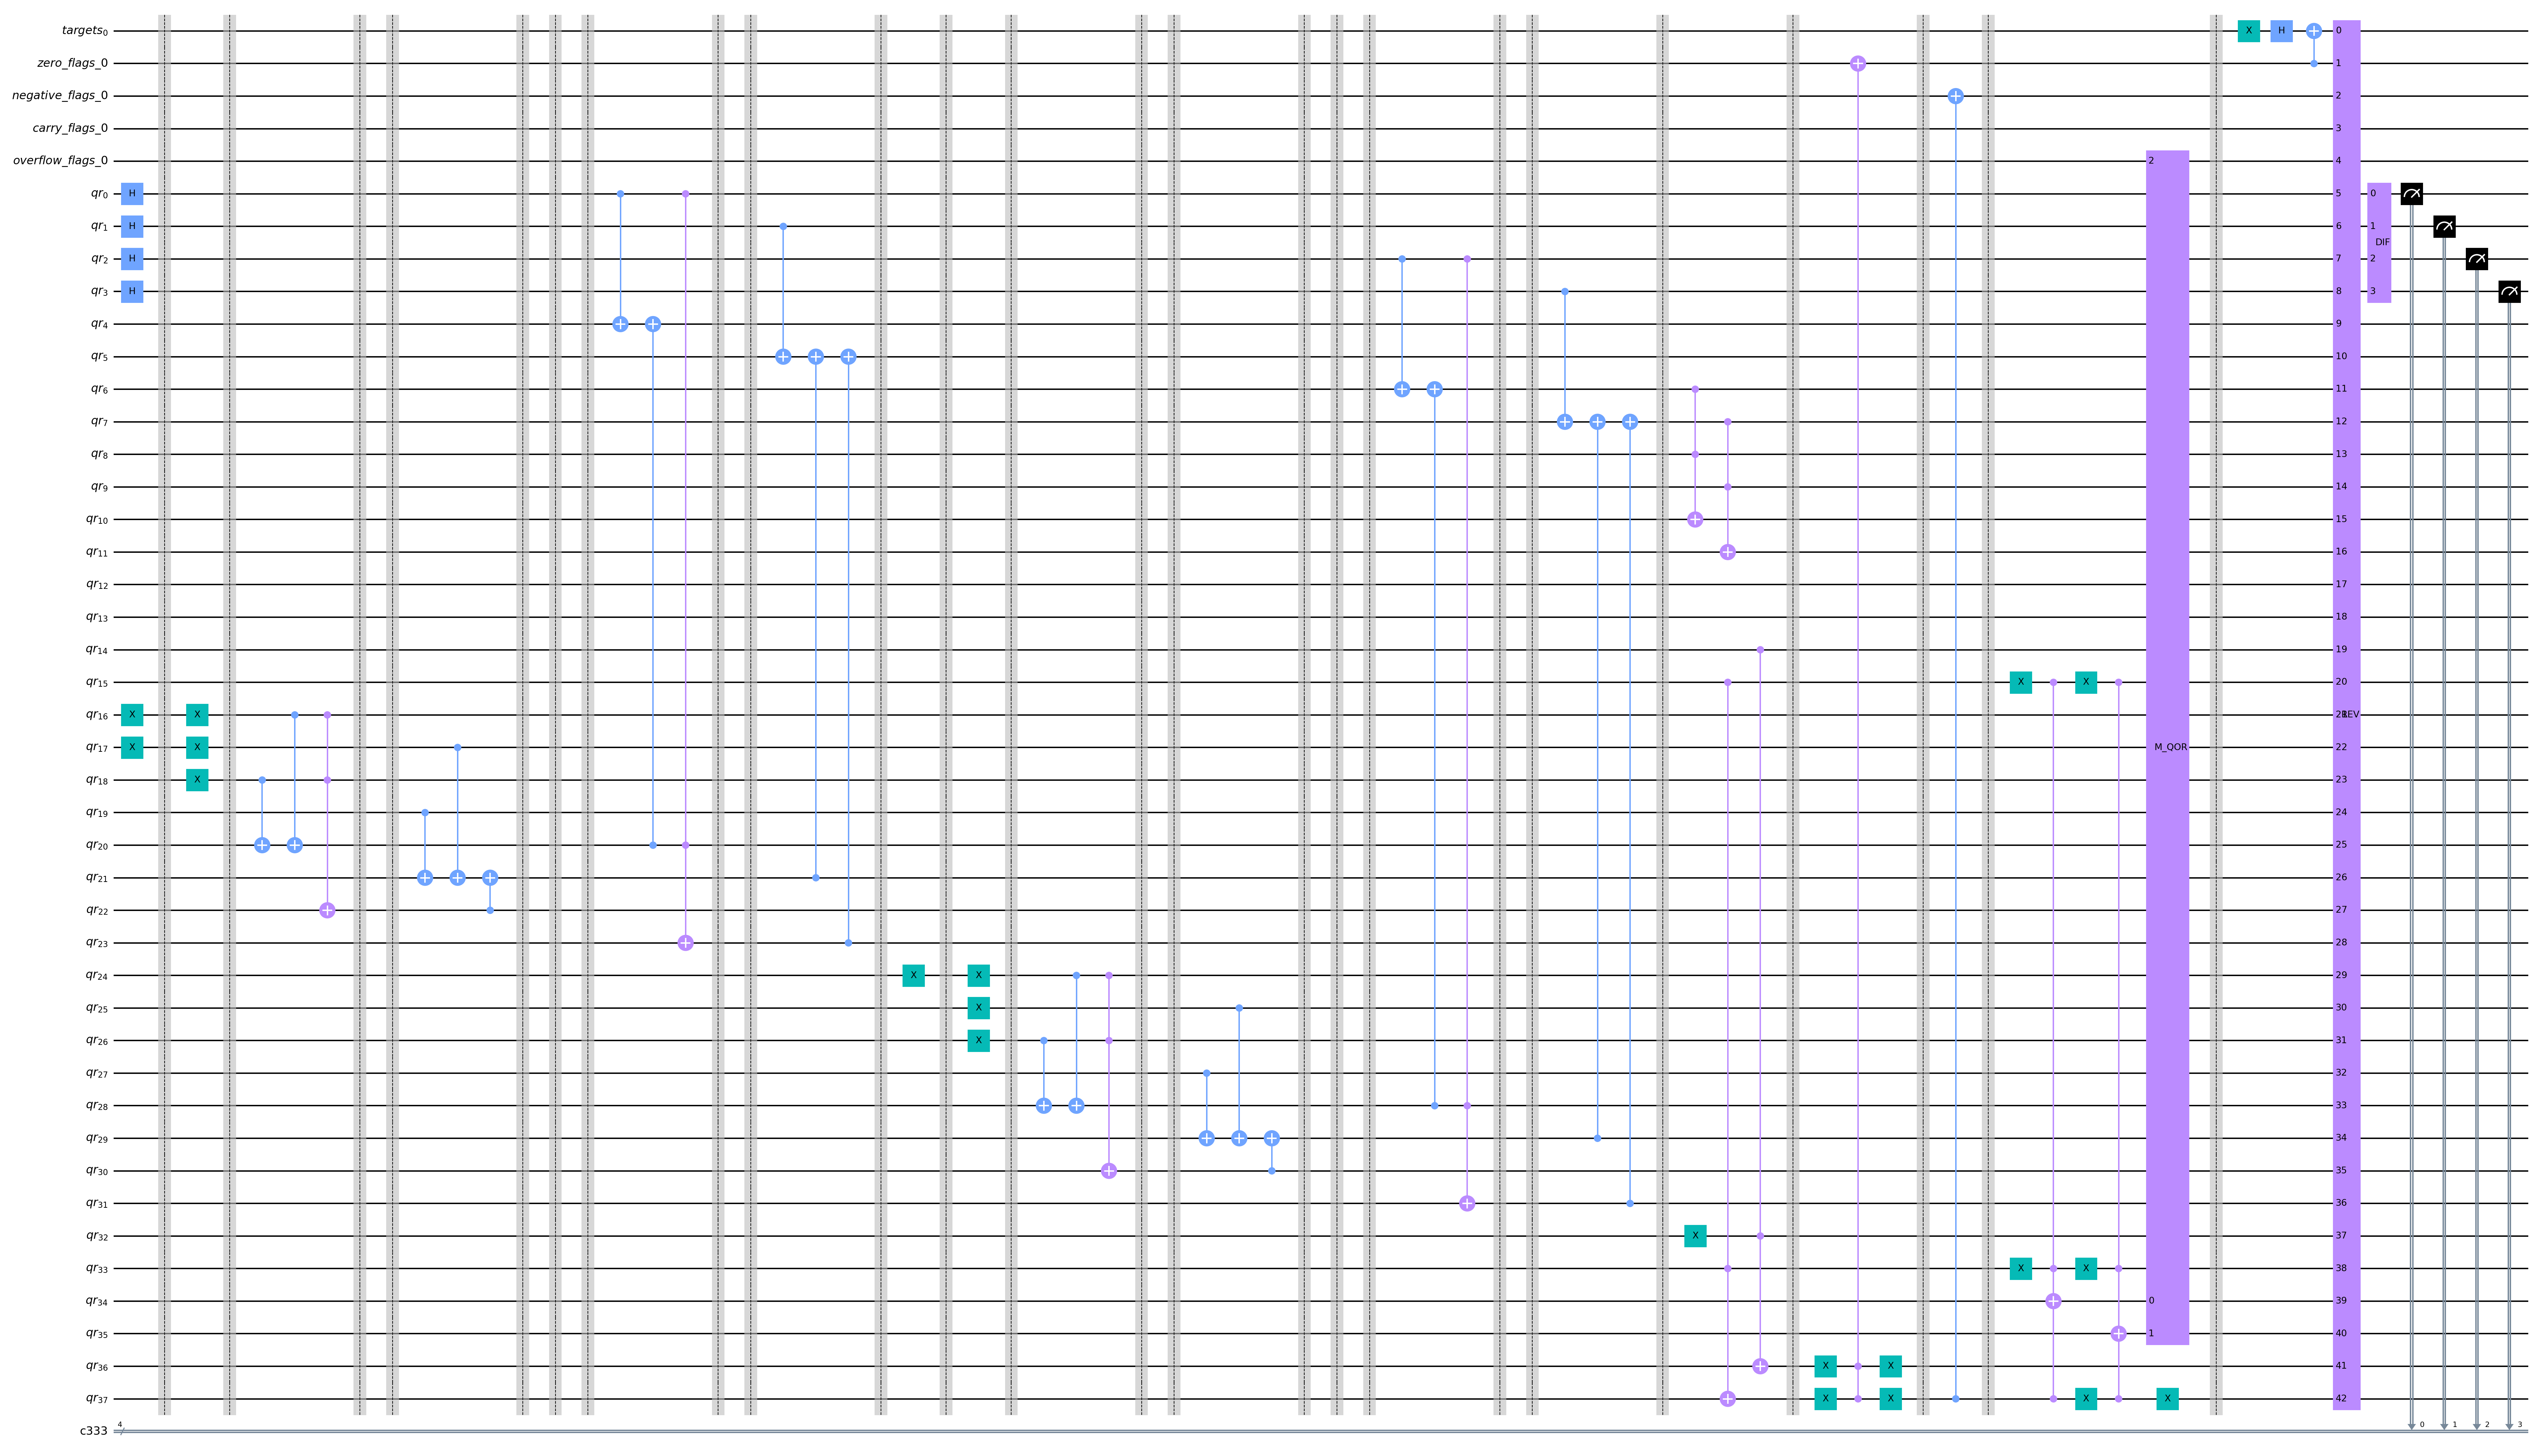
\includegraphics[width=9cm]{Figures/Vehicle_Routing_Problem_circuit.png}
    \caption{Using Grover's Algorithm to Solve the Vehicle Routing Problem Problem}
    \label{fig:Vehicle_Routing_Problem}
\end{figure}

\section{Conclusion}
\label{sec:conclusion}

In this paper, we have presented a novel approach for solving the Vehicle Routing Problem using Grover's Algorithm, a quantum search algorithm known for its quadratic speedup over classical search algorithms. Our approach involves a suitable encoding scheme to represent routes as quantum states and the construction of an oracle to mark the target states corresponding to optimal or near-optimal solutions. We have analyzed the performance of our approach and demonstrated its potential benefits and limitations.

Our proposed method offers a significant advantage over classical techniques in terms of computational complexity and has the potential to efficiently solve large-scale VRP instances and complex variants. However, the current state of quantum computing hardware poses a challenge for the practical implementation of our approach, as the required number of qubits and gates exceeds the capabilities of existing quantum computers. As quantum computing technology advances, we expect that our approach will become increasingly feasible and effective for solving the VRP and related problems.

Future research directions include the investigation of alternative encoding schemes and oracle constructions, as well as the adaptation of our approach to different VRP variants and constraints. Moreover, the integration of our method with other quantum techniques, such as quantum walks and adiabatic quantum computing, may offer additional benefits and further improve the algorithm's performance.

